\begin{frame}
		\frametitle{From STL To Voxels}
		\begin{minipage}{0.85\textwidth}
			Tools:
			\begin{itemize}
			\item Common Versatile Multi-purpose Library for C++ (CVMLCPP)
				\begin{itemize}			
				\item Takes .stl file and returns a binary file with the given voxel size
				\end{itemize}
			\item Custom script to read binary file and output it as ascii.vtk
			\end{itemize}
			\only<1>{			
			\centering
			\begin{figure}
			
\includegraphics[scale=0.15]{Pictures/STLToVoxels/Star_STL.png}
			\end{figure}
			}
			\only<2>{
			\centering
			\begin{figure}
			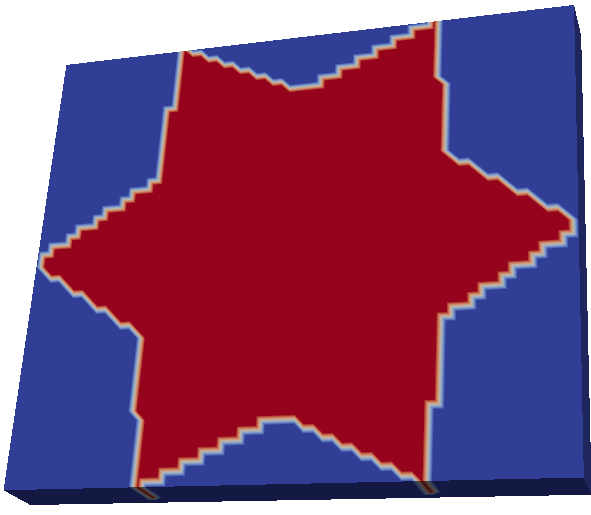
\includegraphics[scale=0.1706]{Pictures/STLToVoxels/Star_VTK_Trans.png}
			\end{figure}
			}
			\only<3>{
			\centering
			\begin{figure}
			
\includegraphics[scale=0.15]{Pictures/STLToVoxels/Star_STL.png}
			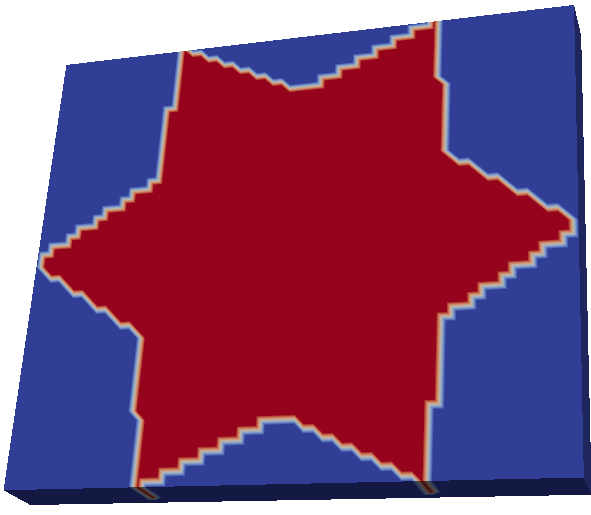
\includegraphics[scale=0.1706]{Pictures/STLToVoxels/Star_VTK_Trans.png}
			\end{figure}
			}
		\end{minipage}
		\begin{minipage}{0.14\textwidth}
			\begin{figure}
				\scalebox{0.08}{
\includegraphics{Pictures/1CAD.pdf}}\\
				\scalebox{0.08}{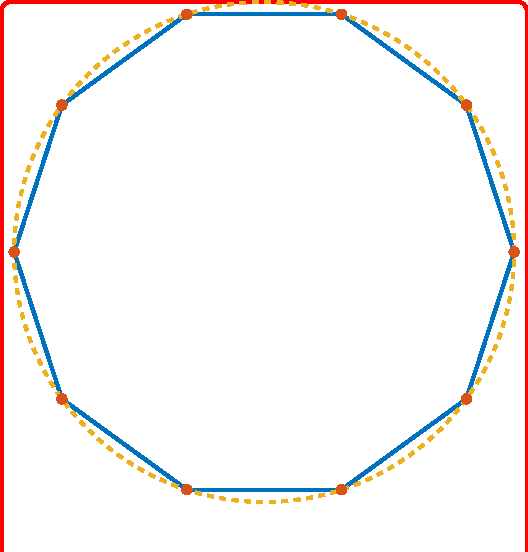
\includegraphics{Pictures/2STLmark2.pdf}}\\
				\scalebox{0.08}{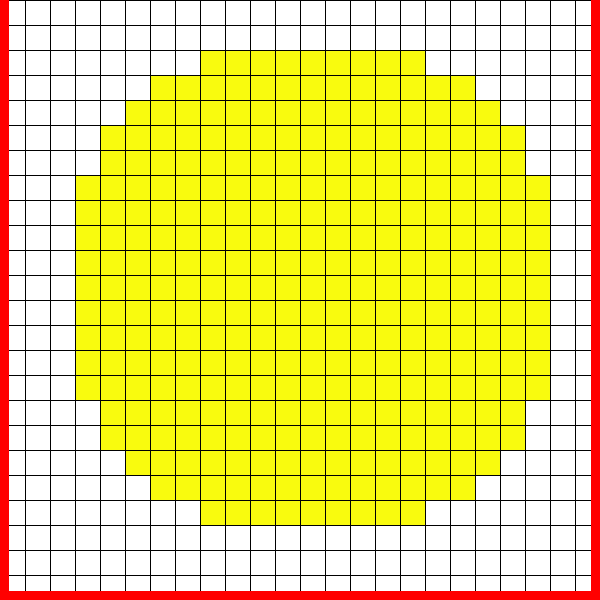
\includegraphics{Pictures/3VOXmark1.pdf}}\\
				\scalebox{0.08}{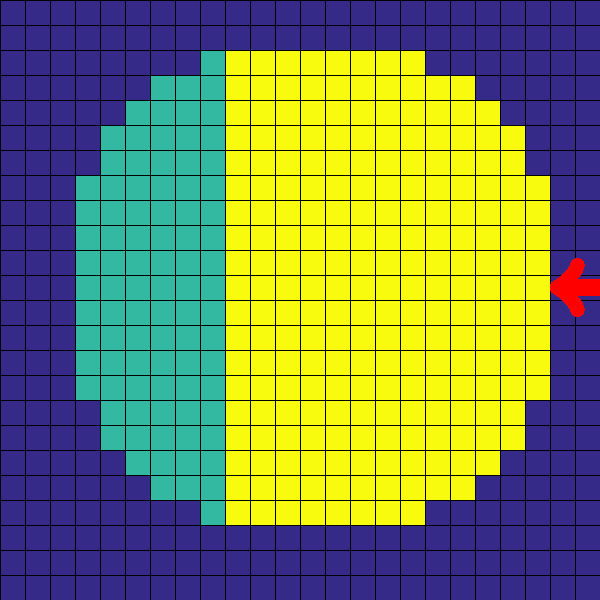
\includegraphics{Pictures/4TPD.pdf}}\\
				\scalebox{0.08}{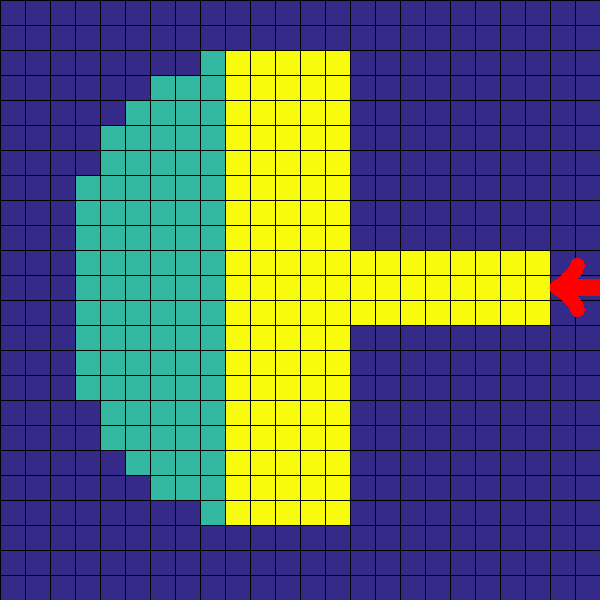
\includegraphics{Pictures/5TOPOPT.pdf}}\\
		%		\scalebox{0.08}{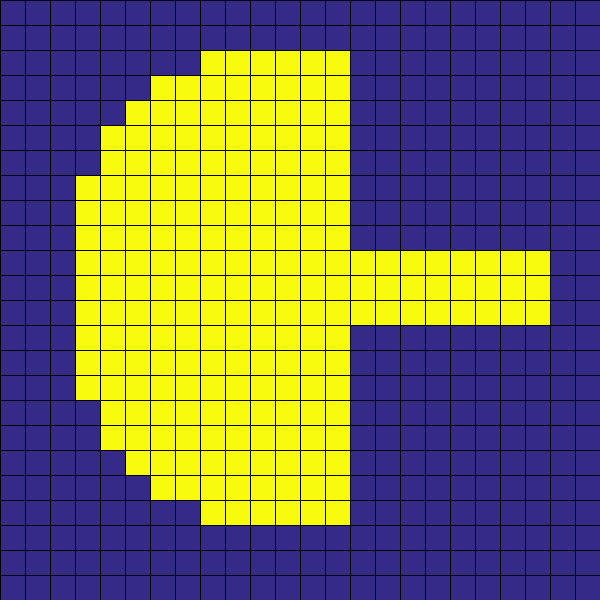
\includegraphics{Pictures/6TOPYOUT.pdf}}\\
				\scalebox{0.08}{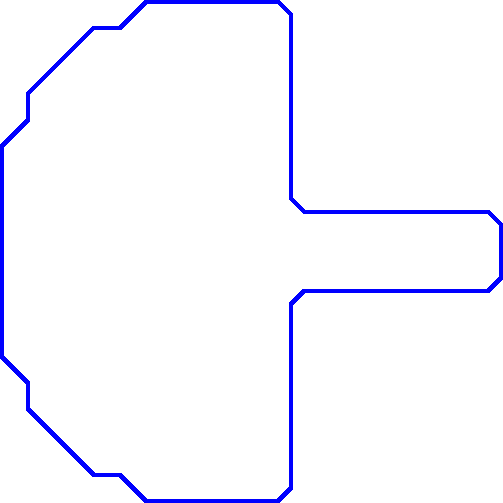
\includegraphics{Pictures/7MC.pdf}}
				\scalebox{0.08}{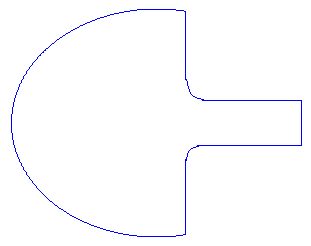
\includegraphics[scale=1.3]{Pictures/End.png}}
			\end{figure}
		\end{minipage}
\end{frame}
